\section{Anexo técnico}
\subsection{Índice Estacional Medio}\label{section:anexo:IEM}

El índice estacional medio (IEM) responde a la necesidad de entender las tendencias y ciclos en el número de cotizantes que da año a año en el SPS. El comportamiento estacional del total de cotizantes llevo a consolidar el IEM para lograr entender de antemano como va a ser el comportamiento anual de los cotizantes en un año típico (Ver Anexo \ref{fig:anexo:glosario}).  

Se utilizó un filtro de \href{https://direct-mit-edu.ezproxy.library.wur.nl/rest/article-abstract/98/2/310/58328/The-Econometrics-of-the-Hodrick-Prescott-Filter?redirectedFrom=PDF}{Hodrick-Prescott} para realizar la descomposición de la serie de tiempo y extraer los multiplicadores mensuales. El gráfico \ref{fig:anexo:ano_tipo_multiplicadores} muestra el IEM para un año típico. El proceso de aplicación del IEM a cada año se realiza siguiendo la ecuación:

\[
C_t^p = C_{1} * I_{t}
\]
donde $C_t^p$ es el número de cotizantes pronosticado como función del IEM en el mes $t$ ($I_{t}$). $C_{1}$ corresponde al número total de cotizantes para Enero. 

\begin{figure}[!h]
    \centering
    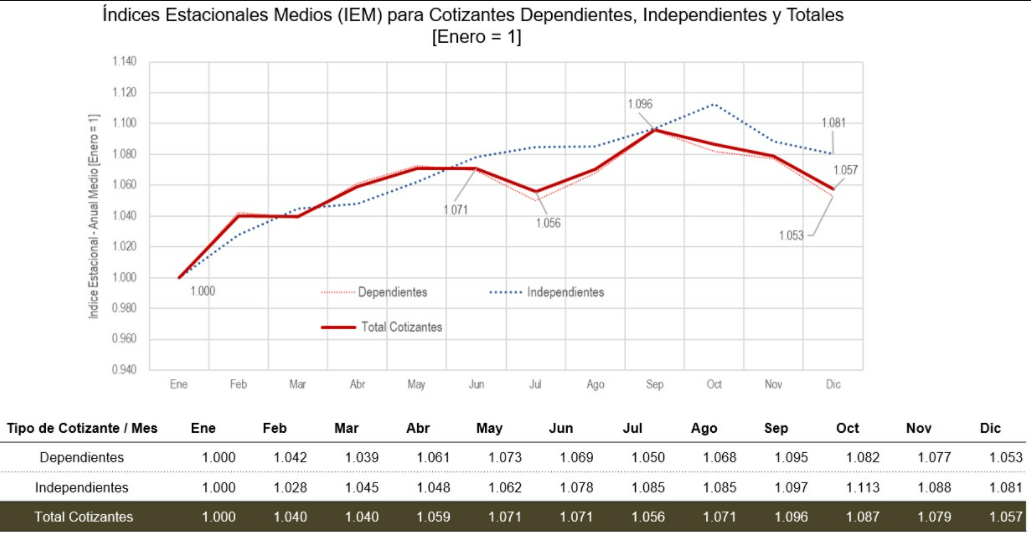
\includegraphics[width = 13cm]{figures/anexo_tecnico/ano_tipo_multiplicadores.png}
    \caption{Índice Estacional Anual Medio}
    \label{fig:anexo:ano_tipo_multiplicadores}
\end{figure}
%\subsection{Cotizantes número 52}
%Gráfico 5. Número de cotizantes tipo 52
%“Beneficiario del mecanismo de protección al cesante” y
%variación anual.
\subsection{Evolución por regímenes}
La figura \ref{fig:anexo:regimenes} muestra el total de personas afiliadas al SPS desagregado por los regímenes contributivo y subsidiado. La razón se interpreta de acuerdo al cociente entre el número de personas del régimen subsidiado y el contributivo. 

\begin{figure}[!htbp]
    \centering
    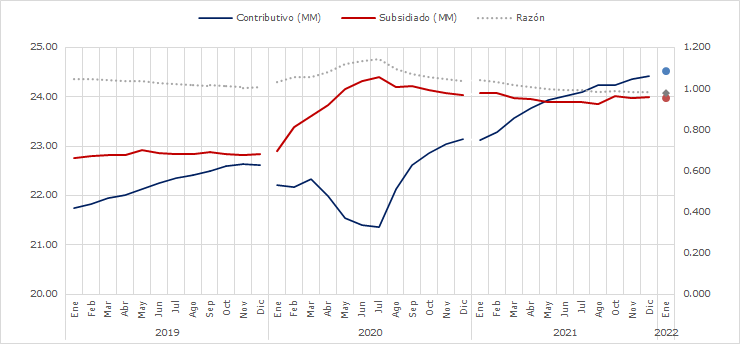
\includegraphics[width = 13cm]{figures/anexo_tecnico/contributivo_subsidiado_regimenes.png}
    \caption{Evolución del total de personas por régimen de afiliación (mill.)}
    \label{fig:anexo:regimenes}
\end{figure}

\FloatBarrier
\subsection{Dinámicas y análisis permanencias}

%%%%%%%%%%%%%%%%%%%%%%%%%%%%%%%%%%%%%%%%%%%%%%%%%%%%%%%%%%%%%%%%%%%%%%%%
%%%%%%%%%%%%%%% DEPENDIENTES %%%%%%%%%%%%%%%%%%%%%%%%%%%%%%%%%%%%%%%%%%%
%%%%%%%%%%%%%%%%%%%%%%%%%%%%%%%%%%%%%%%%%%%%%%%%%%%%%%%%%%%%%%%%%%%%%%%%
\begin{table}[!h]
\centering
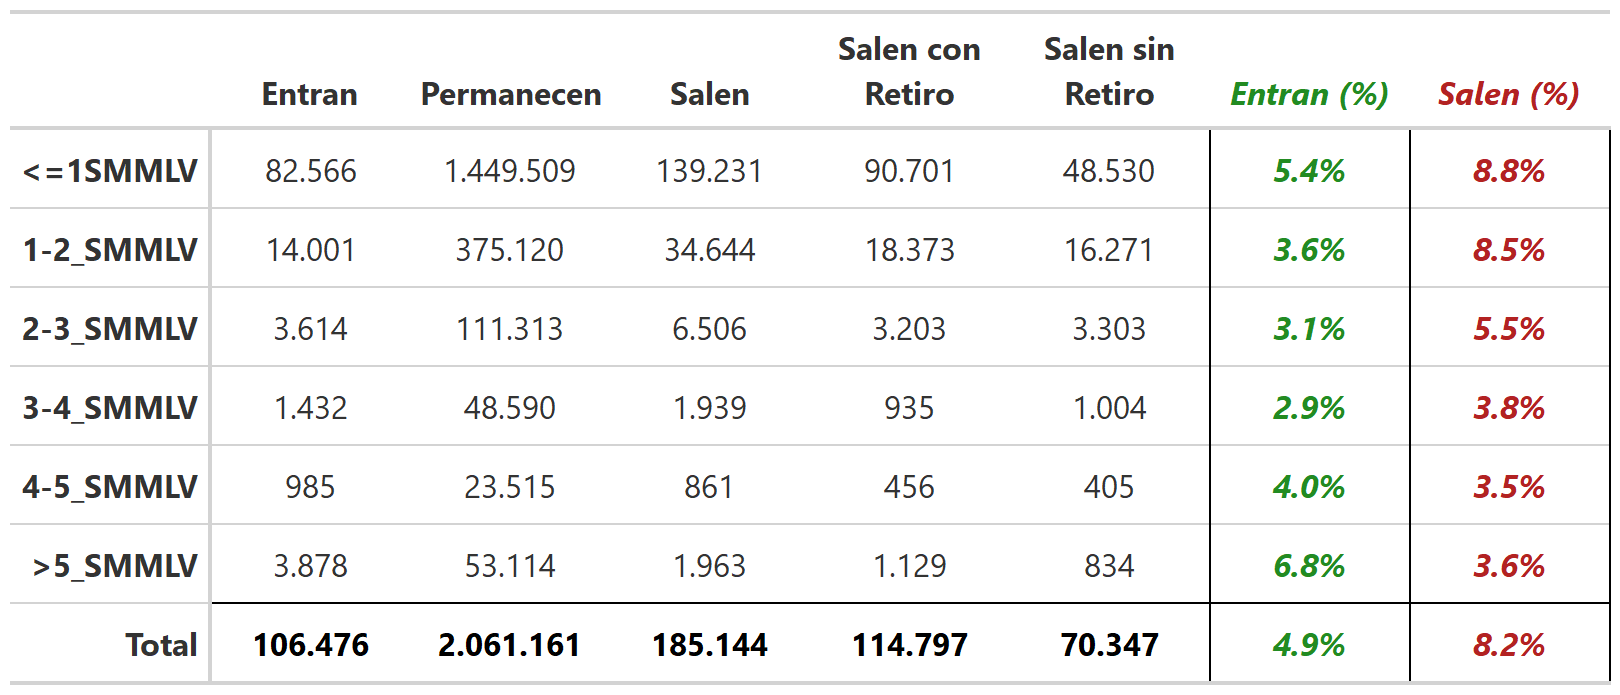
\includegraphics[width = 15cm]{results/02_longitudinal/salida_resumen_dependientes_interes_19.png}
\caption{Matriz dinámica pareada dependientes sector privado Noviembre(filas) - Diciembre(columnas) 2019}%
\label{tabla:sector_privado:matriz_dinamica_mes_interes_19}
\end{table}

\begin{table}[!h]
\centering
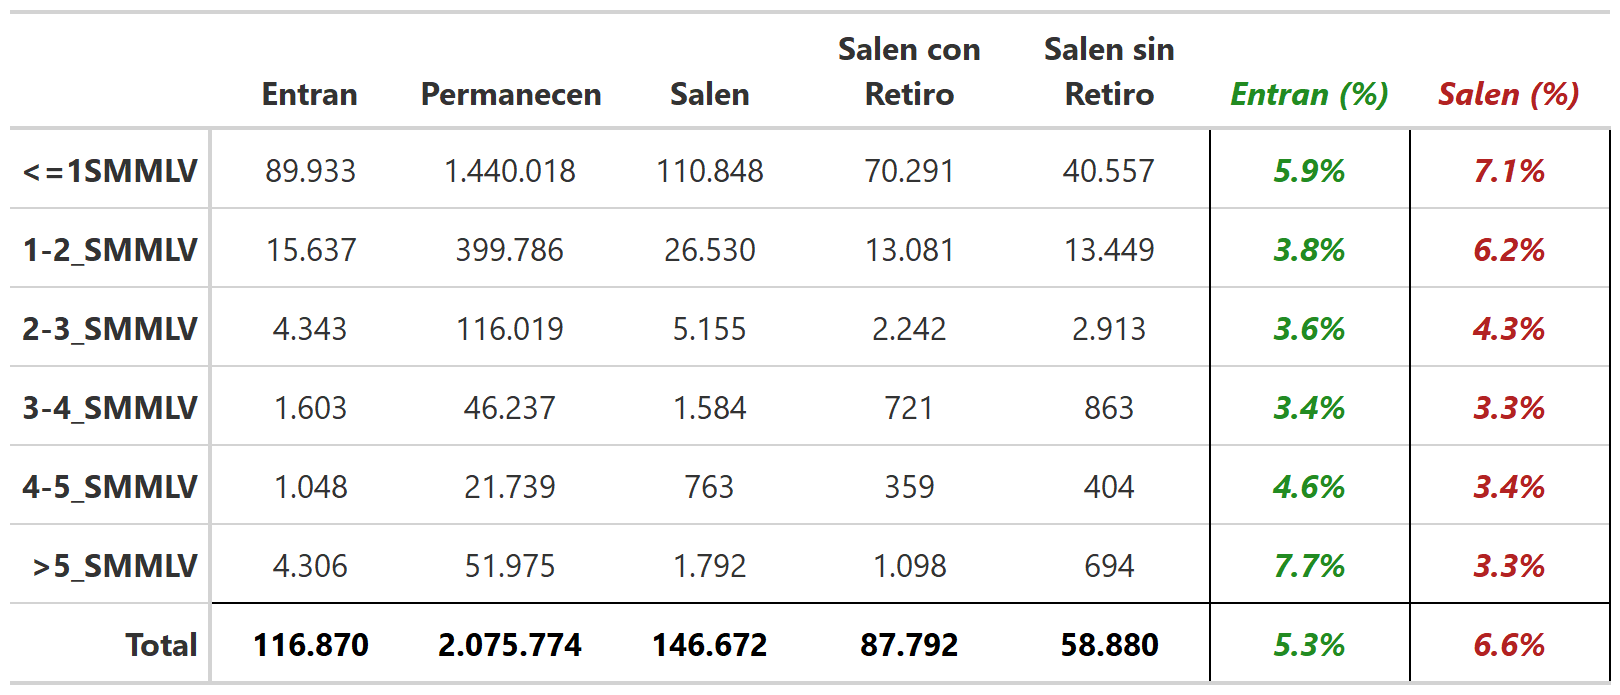
\includegraphics[width = 15cm]{results/02_longitudinal/salida_resumen_dependientes_interes_20.png}
\caption{Matriz dinámica pareada dependientes sector privado Noviembre(filas) - Diciembre(columnas) 2020}%
\label{tabla:sector_privado:matriz_dinamica_mes_interes_20}
\end{table}

\begin{table}[!h]
\centering
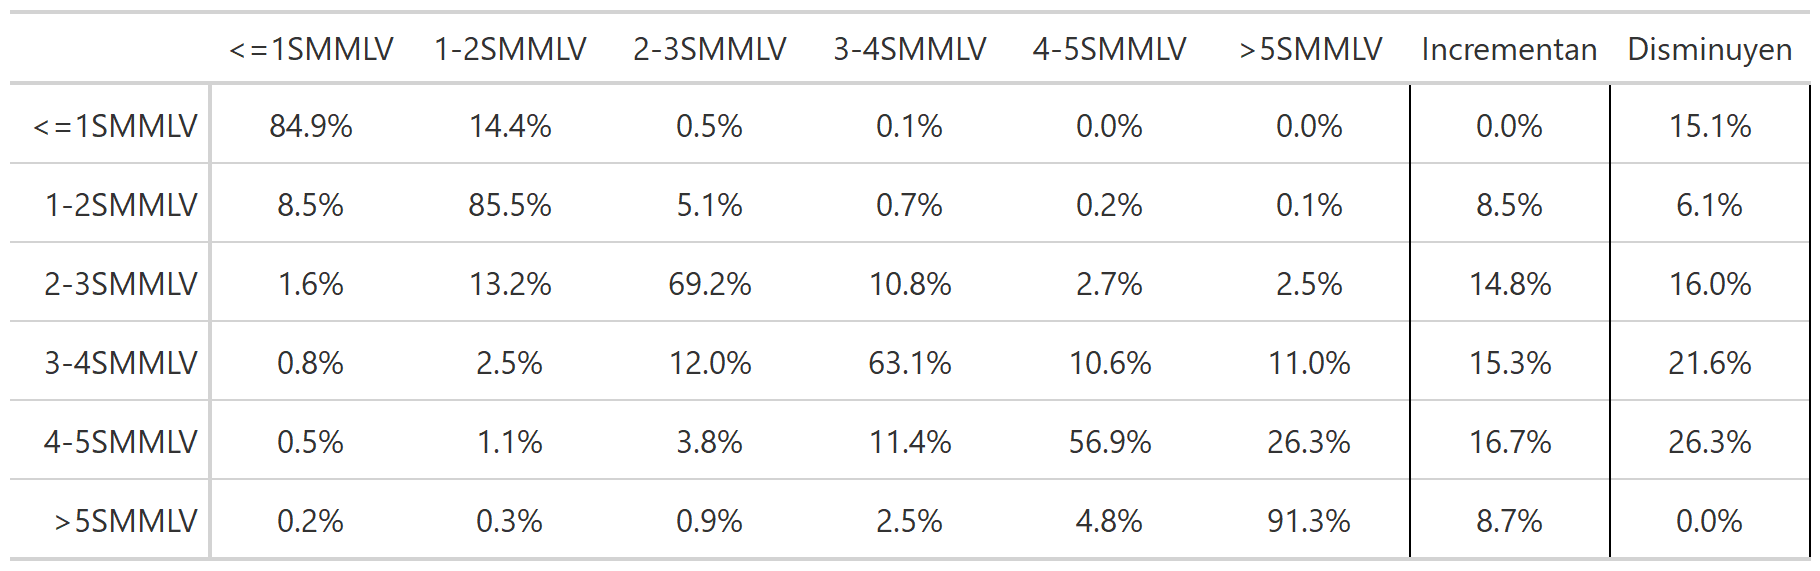
\includegraphics[width = 15cm]{results/02_longitudinal/salida_matriz_transicion_dependientes_19.png}
\caption{Matriz de transición sector privado Noviembre - Diciembre 2019}%
\label{tabla:sector_privado:matriz_transicion_mes_interes_19}
\end{table}

\begin{table}[!h]
\centering
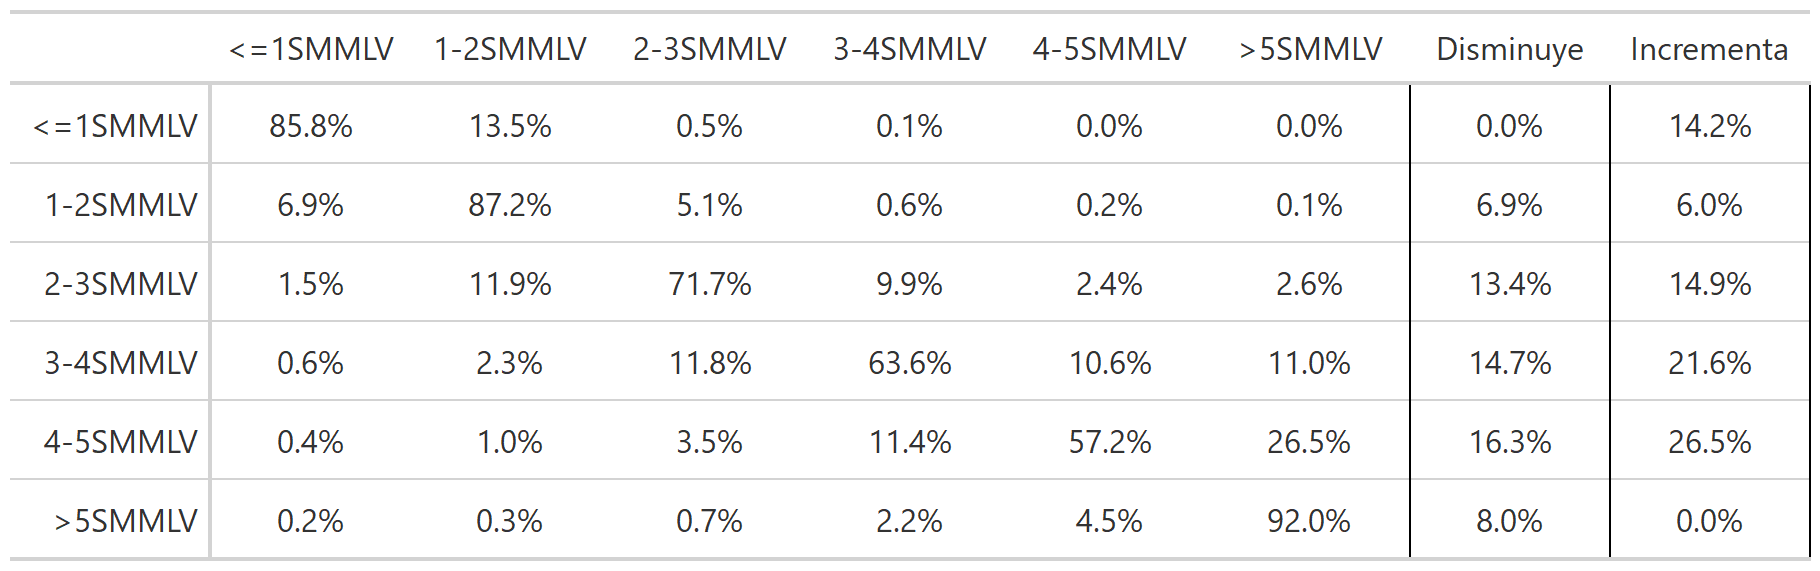
\includegraphics[width = 15cm]{results/02_longitudinal/salida_matriz_transicion_dependientes_20.png}
\caption{Matriz de transición sector privado Noviembre - Diciembre 2020}%
\label{tabla:sector_privado:matriz_transicion_mes_interes_20}
\end{table}



%%%%%%%%%%%%%%%%%%%%%%%%%%%%%%%%%%%%%%%%%%%%%%%%%%%%%%%%%%%%%%%%%%%%%%%%
%%%%%%%%%%%%%%% INDEPENDIENTES %%%%%%%%%%%%%%%%%%%%%%%%%%%%%%%%%%%%%%%%%
%%%%%%%%%%%%%%%%%%%%%%%%%%%%%%%%%%%%%%%%%%%%%%%%%%%%%%%%%%%%%%%%%%%%%%%%

\begin{table}[!h]
\centering
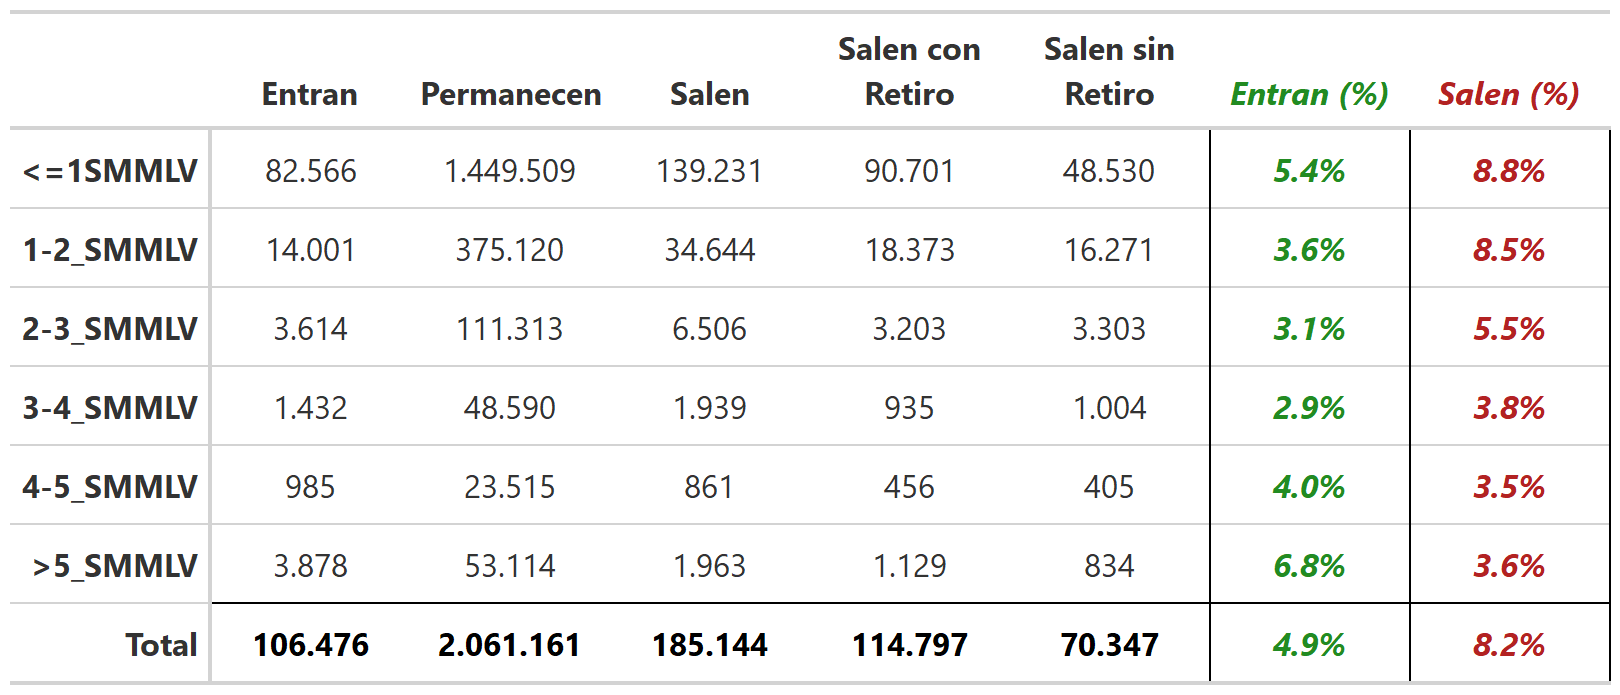
\includegraphics[width = 15cm]{results/02_longitudinal/salida_resumen_independientes_interes_19.png}
\caption{Matriz dinámica pareada independientes Noviembre - Diciembre 2019}%
\label{tabla:independientes:matriz_dinamica_mes_interes_19}
\end{table}

\begin{table}[!h]
\centering
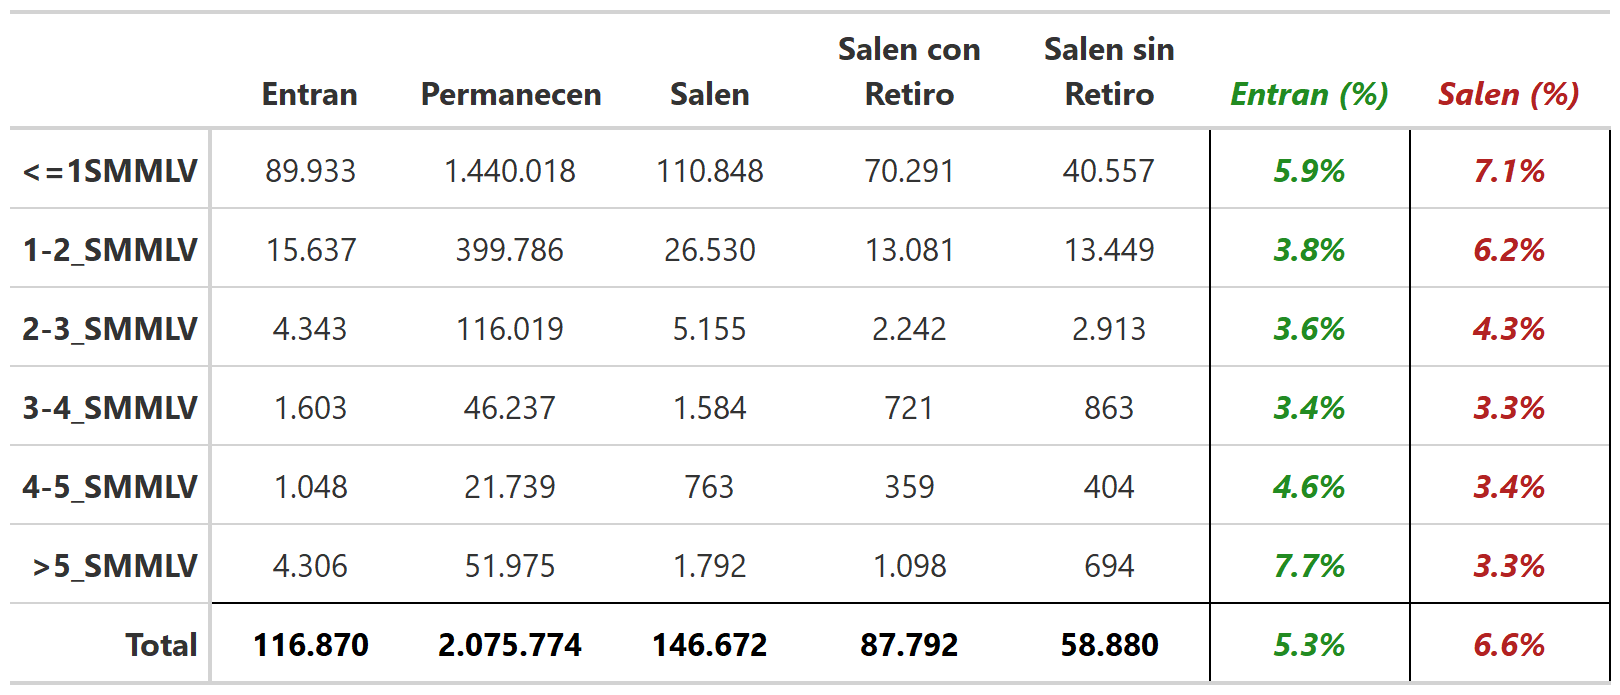
\includegraphics[width = 15cm]{results/02_longitudinal/salida_resumen_independientes_interes_20.png}
\caption{Matriz dinámica pareada independientes Noviembre - Diciembre 2020}%
\label{tabla:independientes:matriz_dinamica_mes_interes_20}
\end{table}

\begin{table}[!h]
\centering
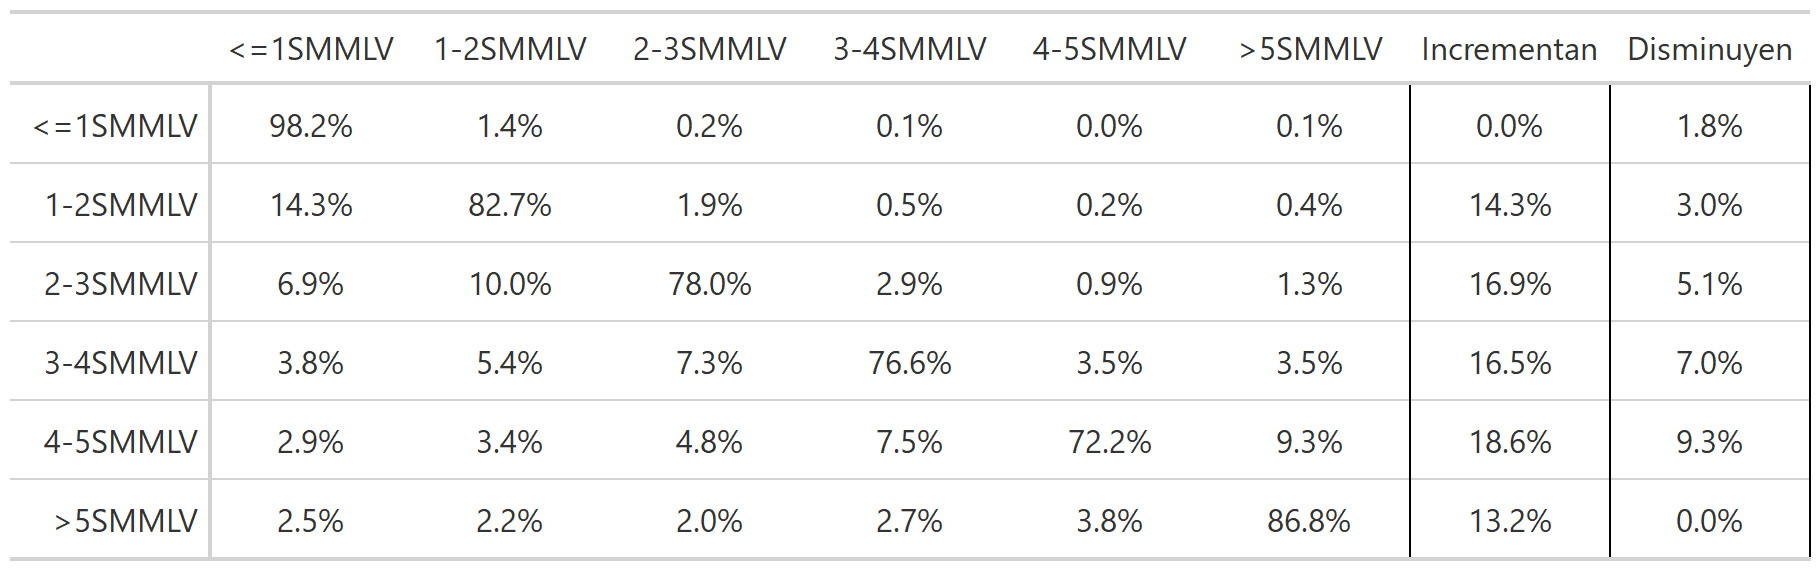
\includegraphics[width = 15cm]{results/02_longitudinal/salida_matriz_transicion_independientes_19.png}
\caption{Matriz de transición independientes Noviembre - Diciembre 2019}%
\label{tabla:independientes:matriz_transicion_mes_interes_19}
\end{table}

\begin{table}[!h]
\centering
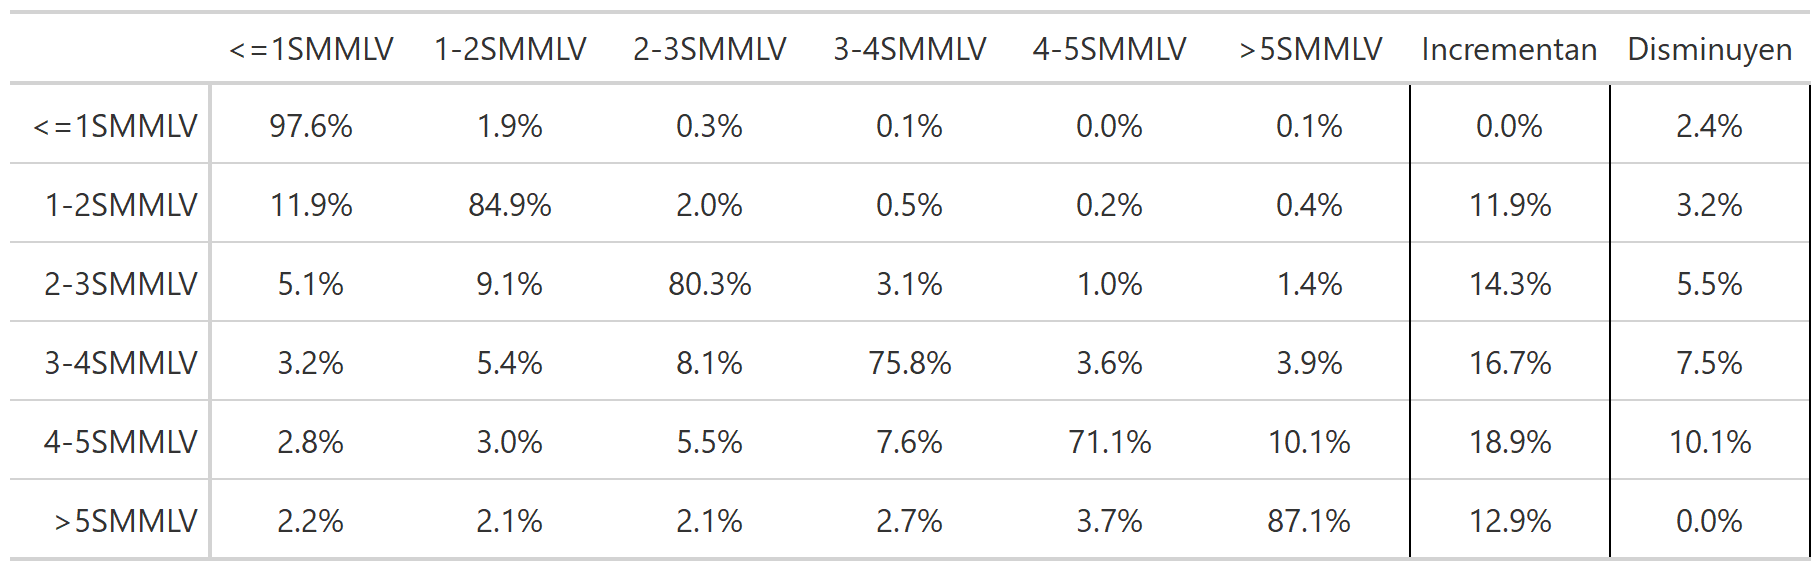
\includegraphics[width = 15cm]{results/02_longitudinal/salida_matriz_transicion_independientes_20.png}
\caption{Matriz de transición independientes Noviembre - Diciembre 2020}%
\label{tabla:independientes:matriz_transicion_mes_interes_20}
\end{table}


%%%%%%%%%%%%%%%%%%%%%%%%%%%%%%%%%%%%%%%%%%%%%%%%%%%%%%%%%%%%%%%%%%%%%%%%
%%%%%%%%%%%%%%% DEMOGRAFICOS %%%%%%%%%%%%%%%%%%%%%%%%%%%%%%%%%%%%%%%%%
%%%%%%%%%%%%%%%%%%%%%%%%%%%%%%%%%%%%%%%%%%%%%%%%%%%%%%%%%%%%%%%%%%%%%%%%

\begin{table}[!h]
\centering
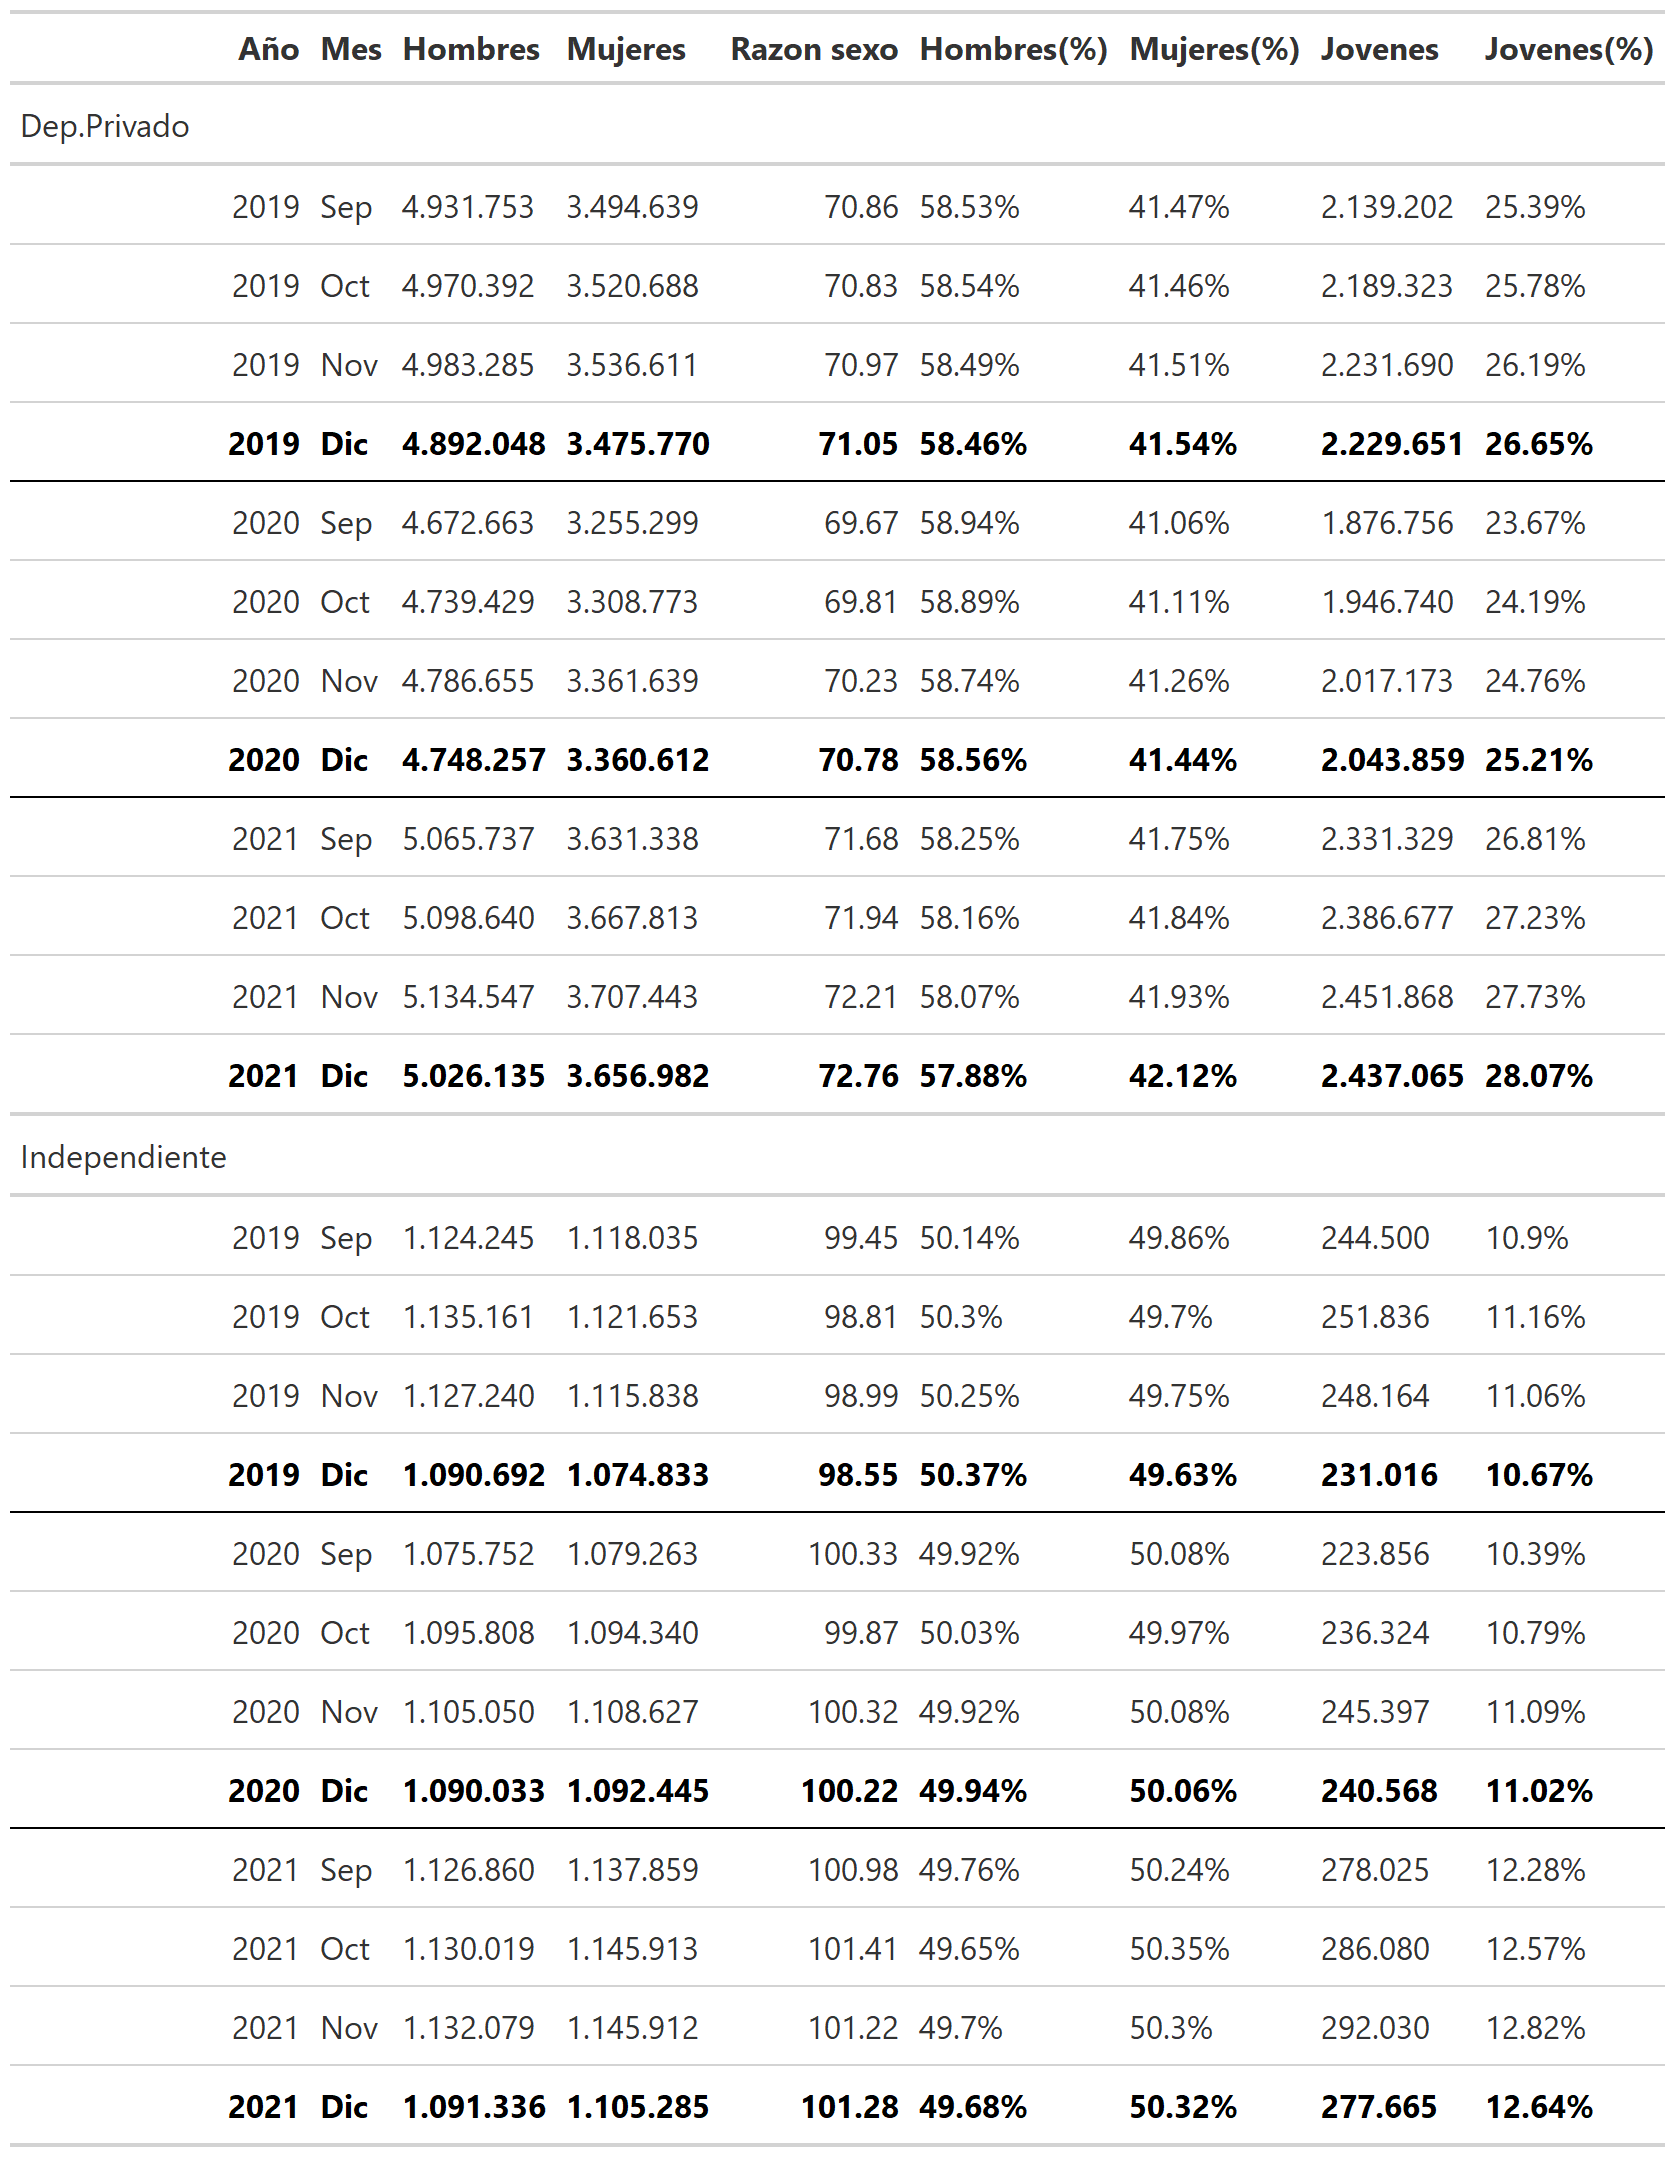
\includegraphics[width = 15cm]{results/02_longitudinal/salida_resumen_demog_dependientes_independientes_21.png}
\caption{Resumen por sexo y edad de transición. Dependientes sector privado e independientes. Noviembre - Diciembre 2019}%
\label{tabla:sector_privado:demograficos}
\end{table}


\FloatBarrier
\subsection{Glosario}\label{fig:anexo:glosario}

\begin{itemize}
    \item \textbf{Aportante:}
    \item \textbf{Ano típico:} El año típico captura las variaciones estacionales a nivel mensual observadas entre 2012 y 2019, con una metodología de descomposición clásica de una serie de tiempo considerando que ésta es una relación multiplicativa entre \textit{tendencia, ciclo, variaciones estacionales y un componente irregular}. Los componentes de la serie de tiempo se obtiene Al observar los momentos de corte en los que se han realizado los análisis hay un retardo de los pagos en los cotizantes independientes
    \item \textbf{Cotizante:} 
    \item \textbf{Cotizante dependiente}
    \item \textbf{Cotizante dependiente del sector privado:}     
    \item \textbf{Cotizante dependiente del sector público:}     
    \item \textbf{Cotizante independientes:}    
    \item \textbf{Ingresos}: Corresponden a las relaciones laborales que para el mes previó al de interés no se encontraban, y fueron identificadas como entradas al SPS para el mes de interés. 
    \item \textbf{Salidas}: Corresponden a las relaciones laborales que para el mes previó al de interés se encontraban en el SPS, y no aparecen registradas en el mes de interés. 
    \item \textbf{Permanencias}: Corresponden a las relaciones laborales que para el mes previó al de interés se encontraban en el SPS, y las cuales aparecen registradas en el mes de interés.     
    \item \textbf{Sección Económica:}         
    \item \textbf{Relación laboral:} 
    \item \textbf{Retiros:}    
    \item \textbf{Vacaciones:}
\end{itemize}



